      
               
                \begin{ledgroupsized}[r]{120mm}
                \footnotesize 
                \pstart                
                \noindent\textbf{\"{U}berlieferung:}   
                \pend
                \end{ledgroupsized}
            
              
                            \begin{ledgroupsized}[r]{114mm}
                            \footnotesize 
                            \pstart \parindent -6mm
                            \makebox[6mm][l]{\textit{LiH}}Marginalien und eine Unterstreichung in \textsc{S. Morland}, \cite{00149}\textit{Tuba stentoro-phonica}, London 1672. \pend
                            \end{ledgroupsized}
                %\normalsize
                \vspace*{5mm}
                \begin{ledgroup}
                \footnotesize 
                \pstart
            \noindent\footnotesize{\textbf{Datierungsgr\"{u}nde}: Das Buch ist 1672 erschienen und der technische Begriff Tubus Morlandi von Leibniz in den Exzerpten aus \textsc{Otto von Guericke}, \cite{00055}\textit{Experimenta nova} (N. 37) erw\"{a}hnt. Leibniz empfiehlt in seinen Textausz\"{u}gen, die Schallausbreitung mit Hilfe dieses Instruments zu untersuchen. Es ist daher von einer Entstehungszeit der Marginalien in der 1. H\"{a}lfte des Jahres 1672 auszugehen.}
                \pend
                \end{ledgroup}
            
                \vspace*{8mm}
                \pstart 
                \normalsize
                %\begin{center}
                %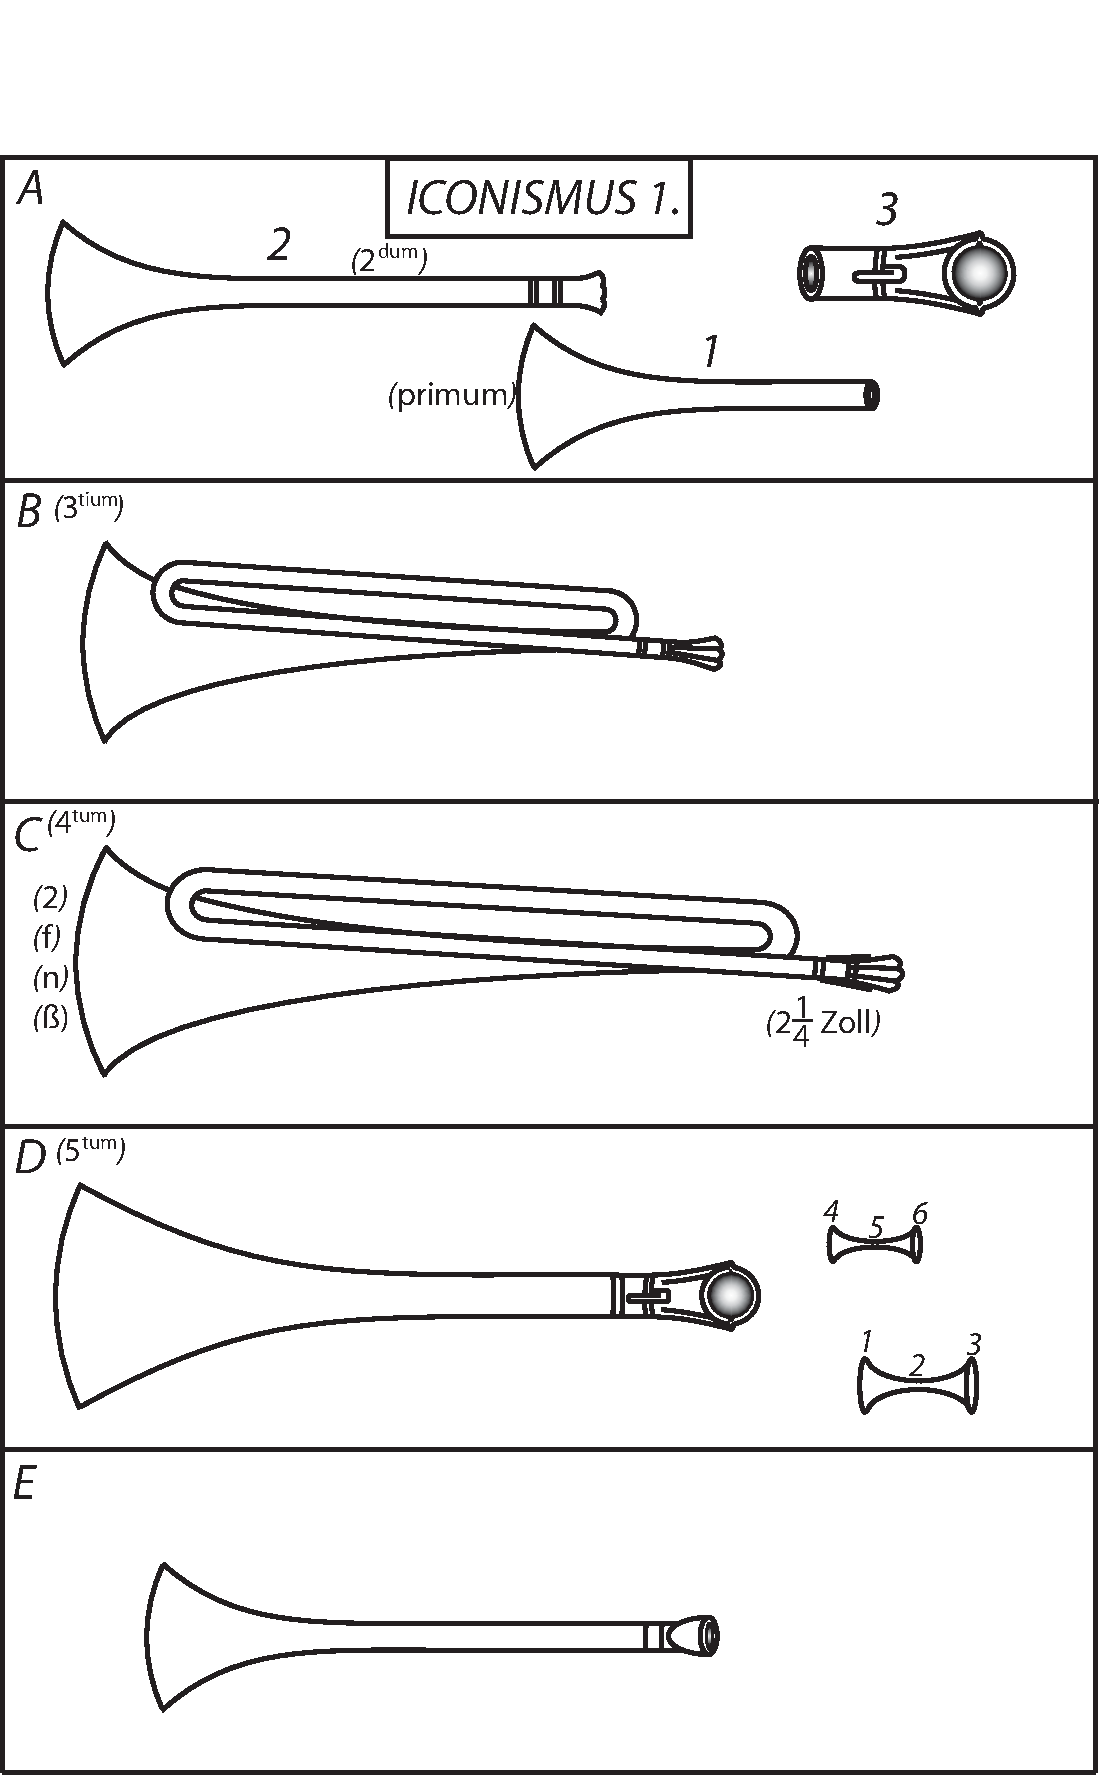
\includegraphics[width=0.45\textwidth]{images/tubus_morlandi.pdf}
                %\\ \textit{[Fig. 1]}
                %\end{center}
                \pend